\documentclass[pdf]{beamer}
\usepackage{booktabs}
\usepackage{comment}
\usepackage{float}
\usepackage{lipsum}
\usepackage{pifont}
 \usepackage[english]{babel}
\usepackage{array}
\usepackage{multirow}
\usepackage{amssymb}
\usepackage{amsthm}
\usepackage{amsmath}
\usepackage[normalem]{ulem}
\usepackage{xspace}
\usepackage{datetime}
\usepackage{hyperref}
\usepackage{textcomp}

\usetheme{Madrid}
\usecolortheme{wolverine}

\newcommand{\tickmark}{\ding{51}}
\newcommand{\xmark}{\ding{55}}

\mode<presentation>{}
\title[The SEA Technique]{Charting a Course Through Uncertain Environments: SEA Uses Past
Problems to Avoid Future Failures}
\author[Moore, Cappos, Frankl, Wies]{Preston Moore, Justin Cappos, Phyllis Frankl, Thomas Wies}
\begin{document}


\begin{frame}
  \titlepage{}
\end{frame}


\begin{frame}{The Problem}
  \begin{itemize}
    \item{Applications work fine during development}
    \item{and then fail in production}
  \end{itemize}
\end{frame}


\begin{frame}{Why does this happen?}
  \begin{figure}
    \centering
    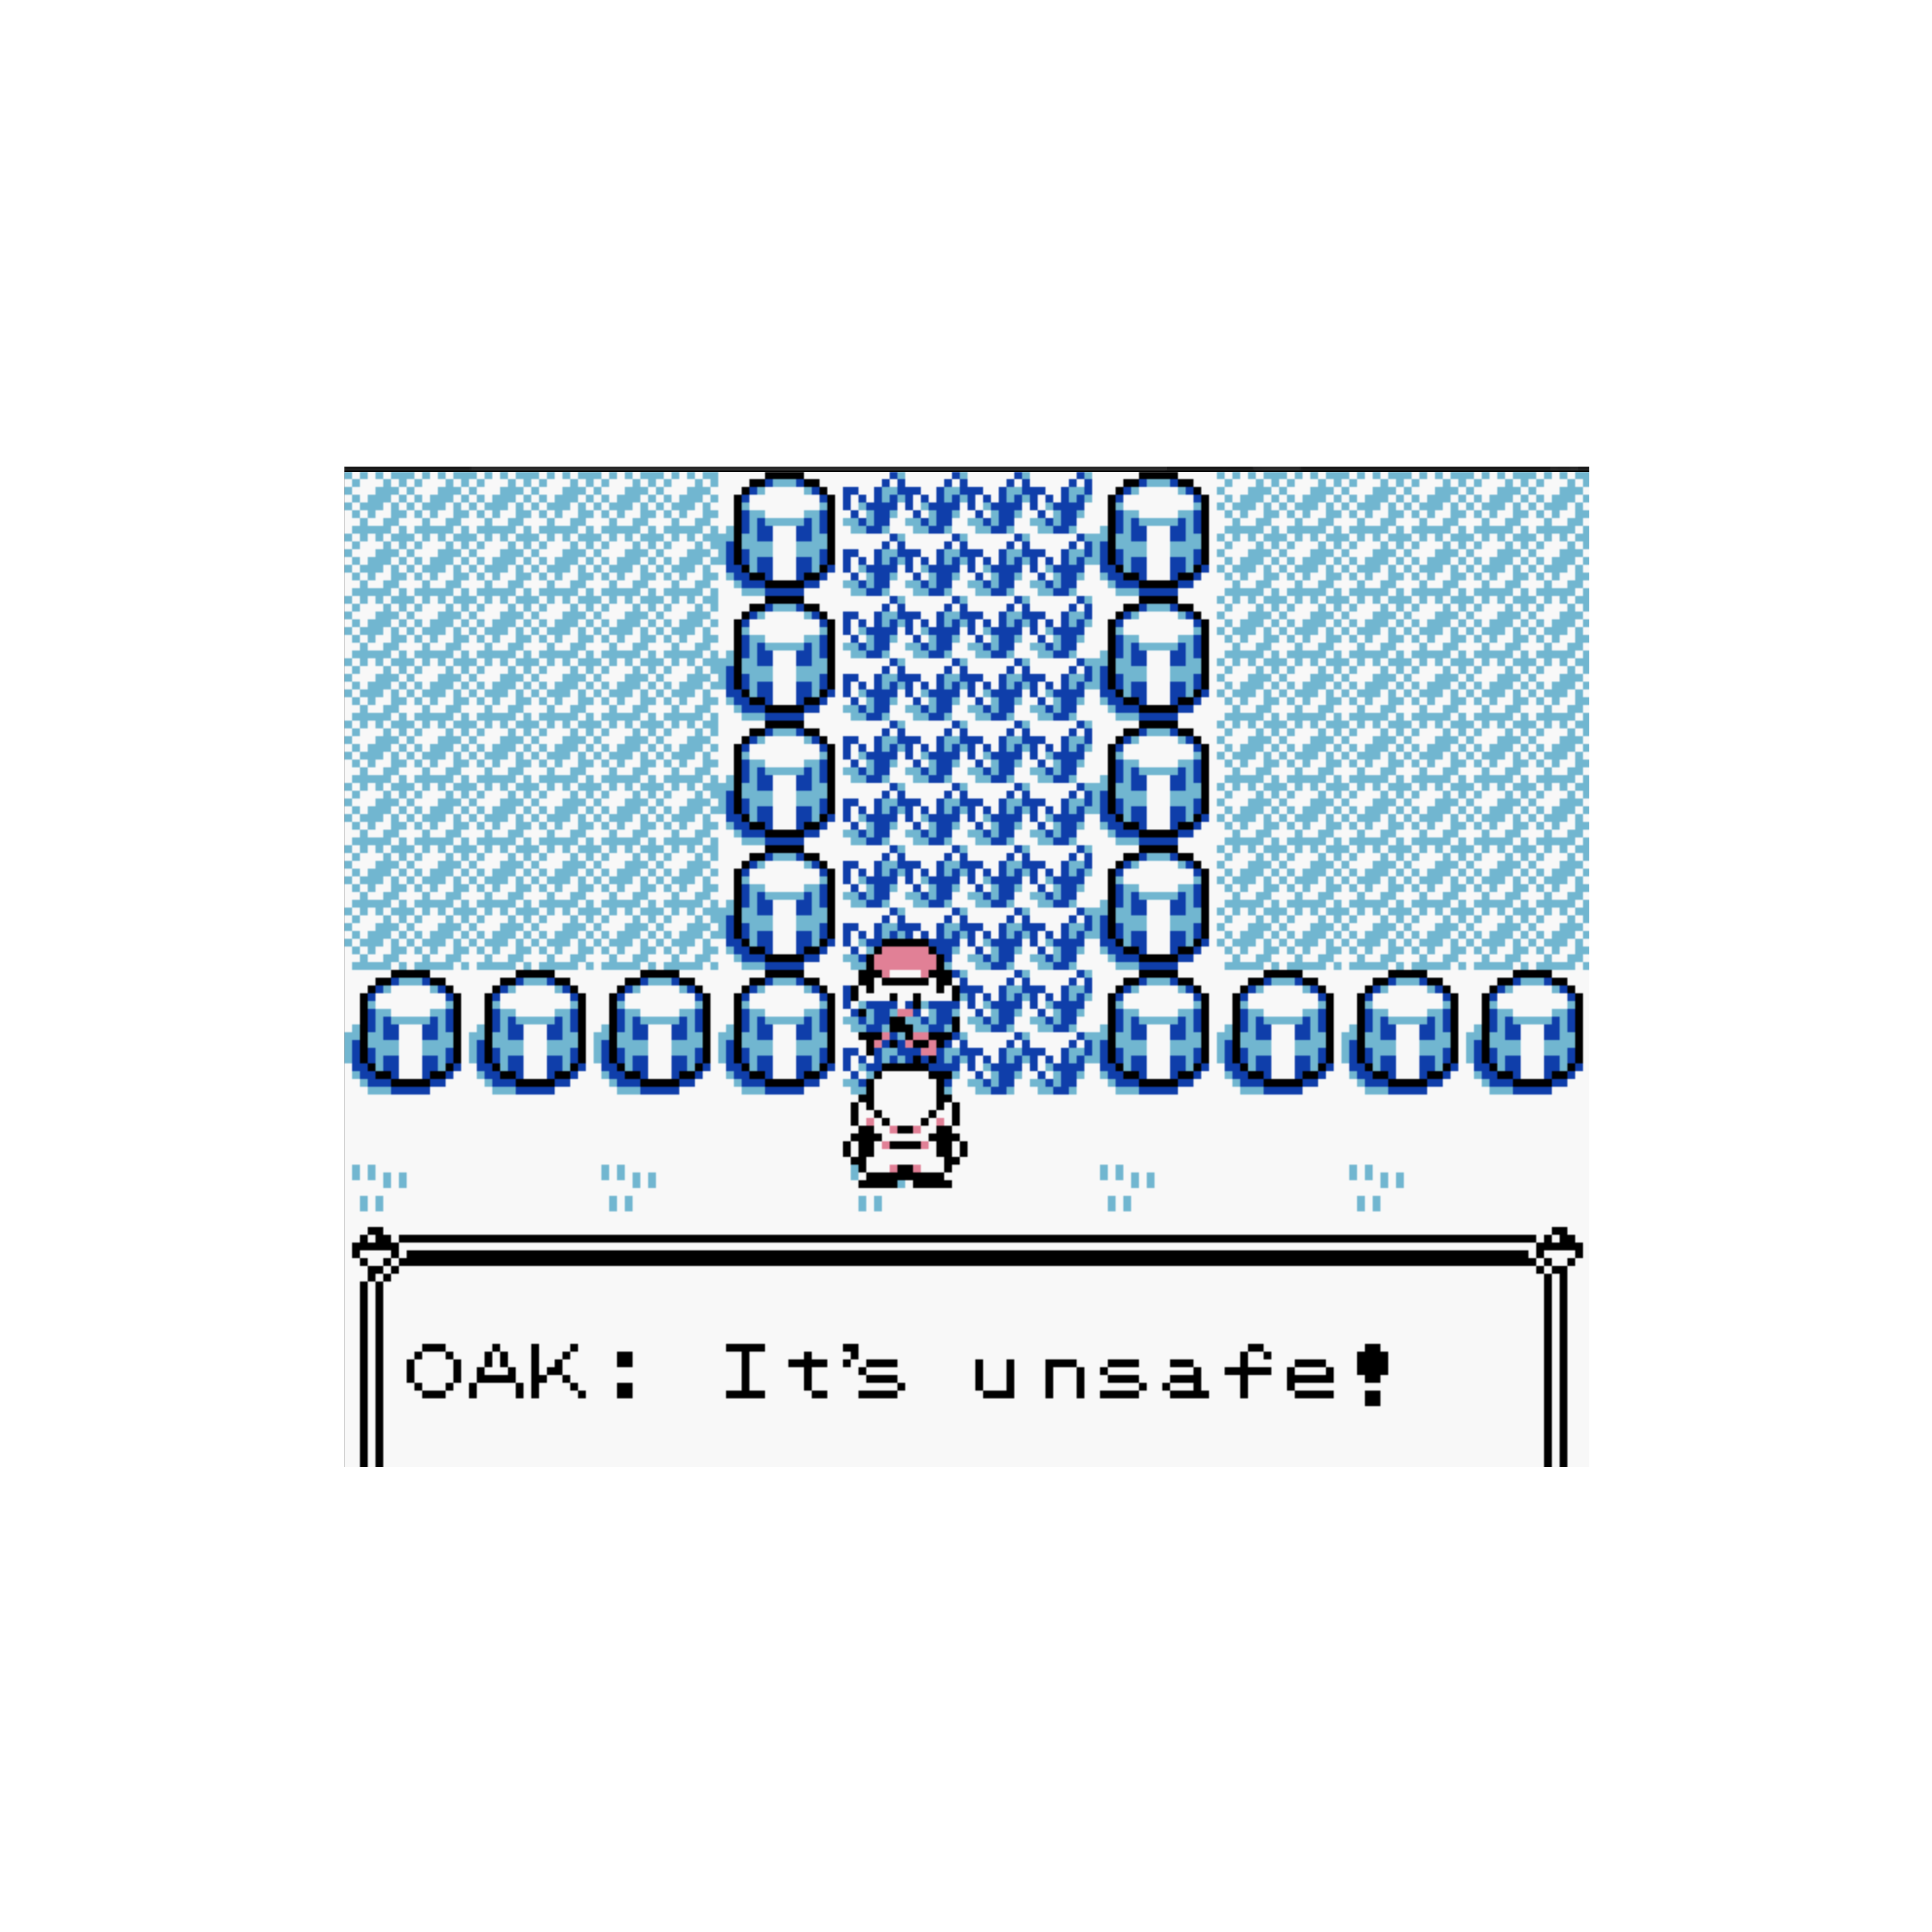
\includegraphics[width = 0.7\textwidth]{images/dangerous}
  \end{figure}
\end{frame}


\begin{frame}{Why does this happen}
  \begin{figure}
    \centering
    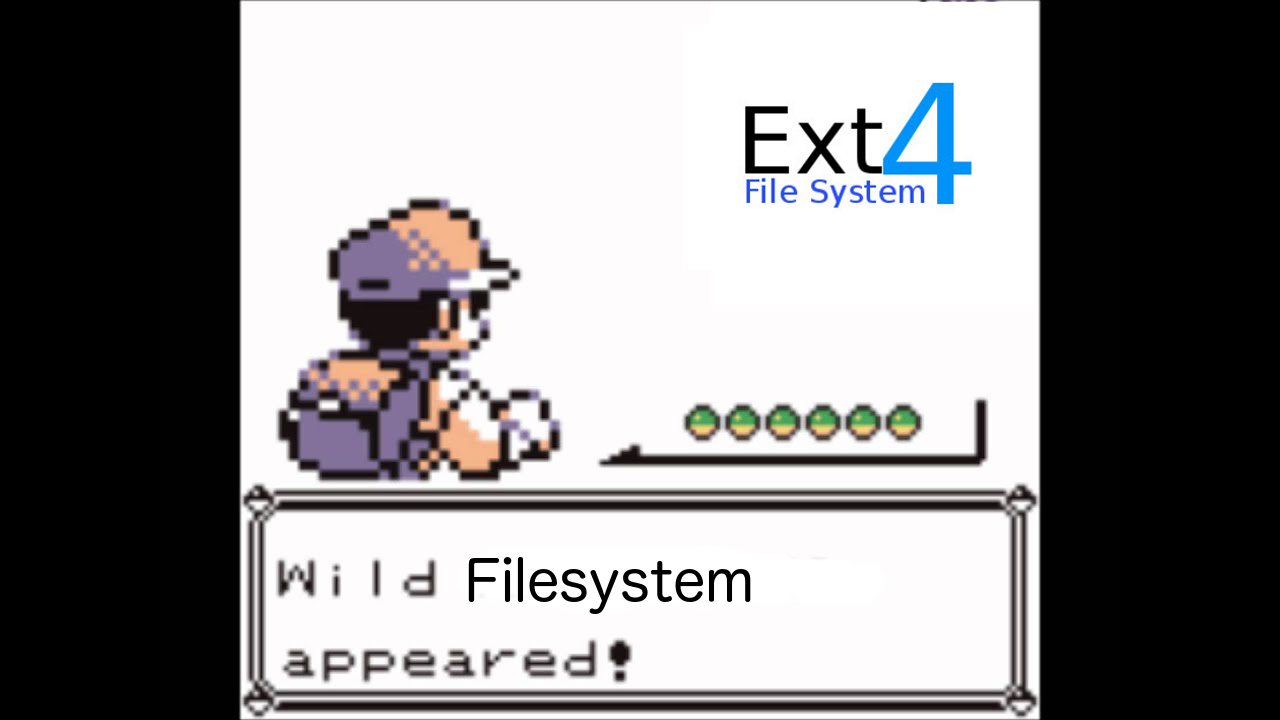
\includegraphics[width = 0.5\textwidth]{images/appears}
  \end{figure}
\end{frame}


\begin{frame}{Why does this happen}
  \begin{figure}
    \centering
    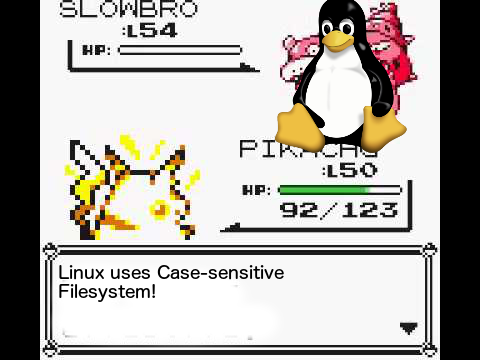
\includegraphics[width = 0.5\textwidth]{images/uses}
  \end{figure}
\end{frame}


\begin{frame}{Why does this happen}
  \begin{figure}
    \centering
    
\includegraphics[width = 0.5\textwidth]{images/supereffective}
  \end{figure}
\end{frame}


\begin{frame}{Deployment Bugs are Frequent and Expensive}
    % Maybe include logos for these organizations/citations etc
    % rather than specific citations
  \begin{itemize}
    % Prevalence
    \item{Oracle: 40\% of deployed applications contain critical flaws}
    \item{A primary cause is differing environments}
    % Cost
    \item{ClusterHQ: 10-25\% of developer time spent on production bugs}
    % We all know how expensive developers are
    % Damage
    \item{Microsoft: 1:1 ratio of testers to developers}
    \item{Google: Recent chrome bug rendered Mac\'s unbootable}
    % But patches still come out that hose machines
  \end{itemize}
\end{frame}


%\begin{frame}{How Does an Environment Influence an Application?}
%  \begin{quote}
%    \LARGE
%    ``I am I and my circumstance...''
%  \end{quote}
%  \hspace*{\fill} --- Jos\'{e} Ortega y Gasset
%\end{frame}


\begin{frame}{How Does an Environment Influence an Application?}
  \begin{itemize}
    \item{An environment is anything out of the developer's control}
    \item{Programs do not execute in isolation}
    \item{Instead, they operate:}
      \begin{itemize}
        \item{On the inputs they are provided}
        \item{\textit{In the context of the environment where they are executed}}
      \end{itemize}
    \item{Developers have become very good at testing applications by
      manipulating inputs}
      \begin{itemize}
        % Environmental influences have not received as much concern
        \item{But environmental influences have not received as much
            concern}
      \end{itemize}
  \end{itemize}
\end{frame}


\begin{frame}{What Does an Environment Provide to an Application?}
  \begin{itemize}
    \item{An implicit input in the form of environment variables, file
      contents, and other data accessible by the application}
    \item{An implementation of the executable resources on which an application depends}
      \begin{itemize}
        \item{e.g. libraries, callable OS functions}
      \end{itemize}
  \end{itemize}
\end{frame}


\begin{frame}{Environments Differ on Many Levels}
  \begin{itemize}
    \item{Versions of libraries and software dependencies}
    \item{Reliability of the network on which the application relies}
    \item{Operating system states, which can vary}
      \begin{itemize}
        \item{\textit{e.g.\ filesystem state, environment variable values}}
      \end{itemize}
  \end{itemize}
\end{frame}


\begin{frame}{Environmental Variations Can Reveal Bugs!}
  % Better define the nature of the problem and the consequences
  An application may fail if:
  \begin{itemize}
    \item{A file it needs is missing}
    \item{It can not handle unusual filesystem configurations}
    \item{It does not handle possible network performance issues}

      % \item{Weird environmental conditions may be uncommon so developers do not
      %   know that they need to handle them!}
  \end{itemize}
  Failure to deal with these conditions results in incorrect behavior --- i.e.\ bugs.

  Identifying these bugs is hard because there are too many variations to
  test against
\end{frame}


\begin{frame}{What is needed...}
  \begin{itemize}
    \item{Is a methodical way to record, preserve, and test against
      problematic environmental features}
  \end{itemize}
\end{frame}


% \begin{frame}{The Typical Deployment Scenario For A New Version of an Application}
%   \begin{itemize}
%   \item{Applications are tested under ideal conditions}
%   \item{Bugs do not present themselves until an application has
%       been deployed to other, less controlled environments}
%   \item{Bugs must then be diagnosed and fixes must be created and distributed}
%   \item{What is needed is a way to test how applications react to particular
%       environmental conditions \textbf{BEFORE} they are deployed}
%   \end{itemize}
% \end{frame}


\begin{frame}{What is needed...}
  \begin{figure}
    \centering
    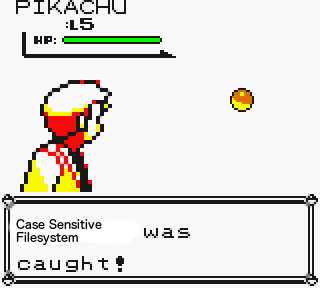
\includegraphics[width = 0.5\textwidth]{images/wascaught}
  \end{figure}
\end{frame}


\begin{frame}{What is needed...}
  \begin{figure}
    \centering
    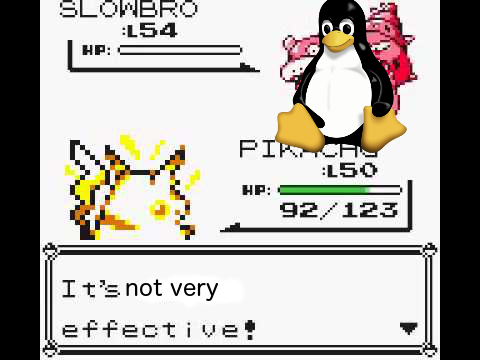
\includegraphics[width = 0.5\textwidth]{images/notveryeffective}
  \end{figure}
\end{frame}


\begin{frame}{Simulating Environmental Anomalies (SEA)}
  \begin{itemize}
    % SEA IS A TECHNIQUE.  Talk about more than just what it does
    \item{SEA captures information about past problems and systematically
        applies it to prevent future failures}
    \item{How it works:}
      \begin{itemize}
        \item{Generically capture and encode unusual environmental
          conditions (referred to as ``anomalies'')}
        \item{Expose a running application to simulated anomalies}
        \item{Assess whether or not the application may be responding this
          simulation}
      \end{itemize}
  \end{itemize}
\end{frame}


\begin{frame}{The Key Ideas}
  \begin{itemize}
    \item{Problematic environmental properties can often be detected in an
      application's}
      \begin{itemize}
        \item{function calls}
        \item{system calls}
        \item{other interactions}
      \end{itemize}
    \item{Exposing an application to these properties gives an idea of how
      likely it is to fail once deployed}
  \end{itemize}
\end{frame}


\begin{frame}{SEA on the Half-Shell}
  % Mention mutators and checkers here so they're good and defined for the
  % next slide

  % To this from the point of view that you have a new application and you
  % want to test it against the repository of prior knowledge of problems
  % from other application
  % Three points here that mirror what we're going to talk about in the
  % design
  \begin{enumerate}
    \item{Record an application as it fails in an anomalous environment}
    \item{Analyze the recording to identify what aspects of the environment
      (known as an anomaly) caused the failure}
    \item{Use this analysis to construct a {\tt mutator} and {\tt checker}}
    \item{Simulate the anomaly on a new application using the mutator}
    \item{Employ the checker in assessing the application's response}

    \item{We simulate real world stuff that has been actually observed}
    \item{Execution tree stuff }
  \end{enumerate}
\end{frame}


\begin{frame}{Generic Example}
  % Specify that delta X does not need to be a integer
  \begin{enumerate}
    \item{An application fails in an environment because problematic
      feature $X$ is present}
    \item{$X$ is analyzed to determine how it causes environmental
      interactions to differ (we call this difference $\Delta X$)}
    \item{$\Delta X$ is used to construct a mutator \textit{mutX()} and
      a checker \textit{checkX()}}
    \item{\textit{mutX()} is used to mutate the system calls of other
      applications in order to simulate the presence of $X$}
    \item{\textit{checkX()} is used to evaluate the application's response
      to $X$}
  \end{enumerate}
\end{frame}


\begin{frame}{An Concrete Example - Simulating the ``Absence'' of a File}
  \begin{itemize}
    \item{Consider an application that depends on reading from file F}
  \end{itemize}

  Normal open: open(F) = 3

  File is missing: open(F) = -1 ENOENT

  \begin{itemize}
    \item{In this case:}
      \begin{itemize}
        \item{$X$ is the fact that F is missing}
        \item{$\Delta X$ is changing the result of open to -1 ENOENT}
        \item{\textit{mutX()} modifies the result of open() calls of another
          application to return -1 ENOENT}
        \item{\textit{checkX()} determines whether the application has
          recognized the failing return value}
      \end{itemize}
  \end{itemize}
\end{frame}


\begin{frame}{Implementing SEA}
  \begin{itemize}
    \item{Identifying and Encoding Anomalies}
    \item{Mutating System Call Results}
    \item{Assessing the Application's Response}
  \end{itemize}
\end{frame}


\begin{frame}{Step 1: Identifying and Encoding Anomalies}
  \begin{itemize}
    \item{An anomaly is found by:}
      \begin{itemize}
        \item{Examining previous failures in the target environment}
        \item{Mining public bug trackers}
        \item{Exploring the output of other tools that find bugs in other
          domains}
      \end{itemize}
    \item{Set of modifications needed to simulate is generated from anomaly}
    \item{Modifications are used to construct a checker and mutator}
    \item{Similar amount of effort to constructing a unit test}
  \end{itemize}
\end{frame}


\begin{frame}{Implementing SEA}
  \begin{itemize}
    \item{Identifying and Encoding Anomalies}
    \item{\textrightarrow{}Mutating System Call Results\textleftarrow{}}
    \item{Assessing the Application's Response}
  \end{itemize}
\end{frame}


\begin{frame}{Step 2: Mutating System Call Results}
  \begin{itemize}
    \item{Execute application while monitoring its system call activity}
    \item{Mutator receives system calls as they occur and watches for pattern
      indicative of a simulation opportunity}
    \item{Once the opportunity arrives, mutator modifies results and side effects
      in order to simulate the anomaly}
  \end{itemize}
\end{frame}


\begin{frame}{Implementing SEA}
  \begin{itemize}
    \item{Identifying and Encoding Anomalies}
    \item{Mutating System Call Results}
    \item{\textrightarrow{}Assessing the Application's Response\textleftarrow{}}
  \end{itemize}
\end{frame}


\begin{frame}{Step 3: Assessing the Application's Response}
  \begin{itemize}
    \item{Checker begins monitoring subsequent system call activity
      after anomaly is simulated}
    \item{Checker either accepts or rejects the execution based on the system
      call activity it observes}
    \item{The specifics of what is accepted or rejected depends on the nature
      of the anomaly being simulated}
  \end{itemize}
\end{frame}


\begin{frame}{Additional Features}
  %  Move up to be part of SEA rather than CrashSimulator
  \begin{itemize}
    \item{Default Checker}
    \item{Accepts or rejects executions based on whether or not the
      application has changed its behavior in response to an anomaly}
      \begin{itemize}
        \item{Changed behavior: possibly addressing anomaly: accept}
        \item{No change: anomaly not recognized: reject}
        \item{This distinction proved sufficient in the majority of cases}
      \end{itemize}
  \end{itemize}
\end{frame}


\begin{frame}{Additional Features}
  \begin{itemize}
    \item{Null Mutator}
      \begin{itemize}
        \item{Performs no mutation but provides opportunity for a checker to
          evaluate an unmodified execution}
      \end{itemize}
  \end{itemize}
\end{frame}


\begin{frame}{CrashSimulator: A Proof of Concept SEA Implementation}

  Implementation Building Blocks:

  \begin{itemize}
    \item{32-bit Linux}
    \item{Modified version rr record-and-replay debugger}
    \item{Python Process Supervisor}
    \item{C Python Module}
      \begin{itemize}
        \item{Manipulation of System Calls using Ptrace}
        \item{Structuring Data}
      \end{itemize}
  \end{itemize}
\end{frame}


\begin{frame}{CrashSimulator's Architecture}
  % Colored box tracking the pieces we're talking about
    \begin{figure}
    \centering
    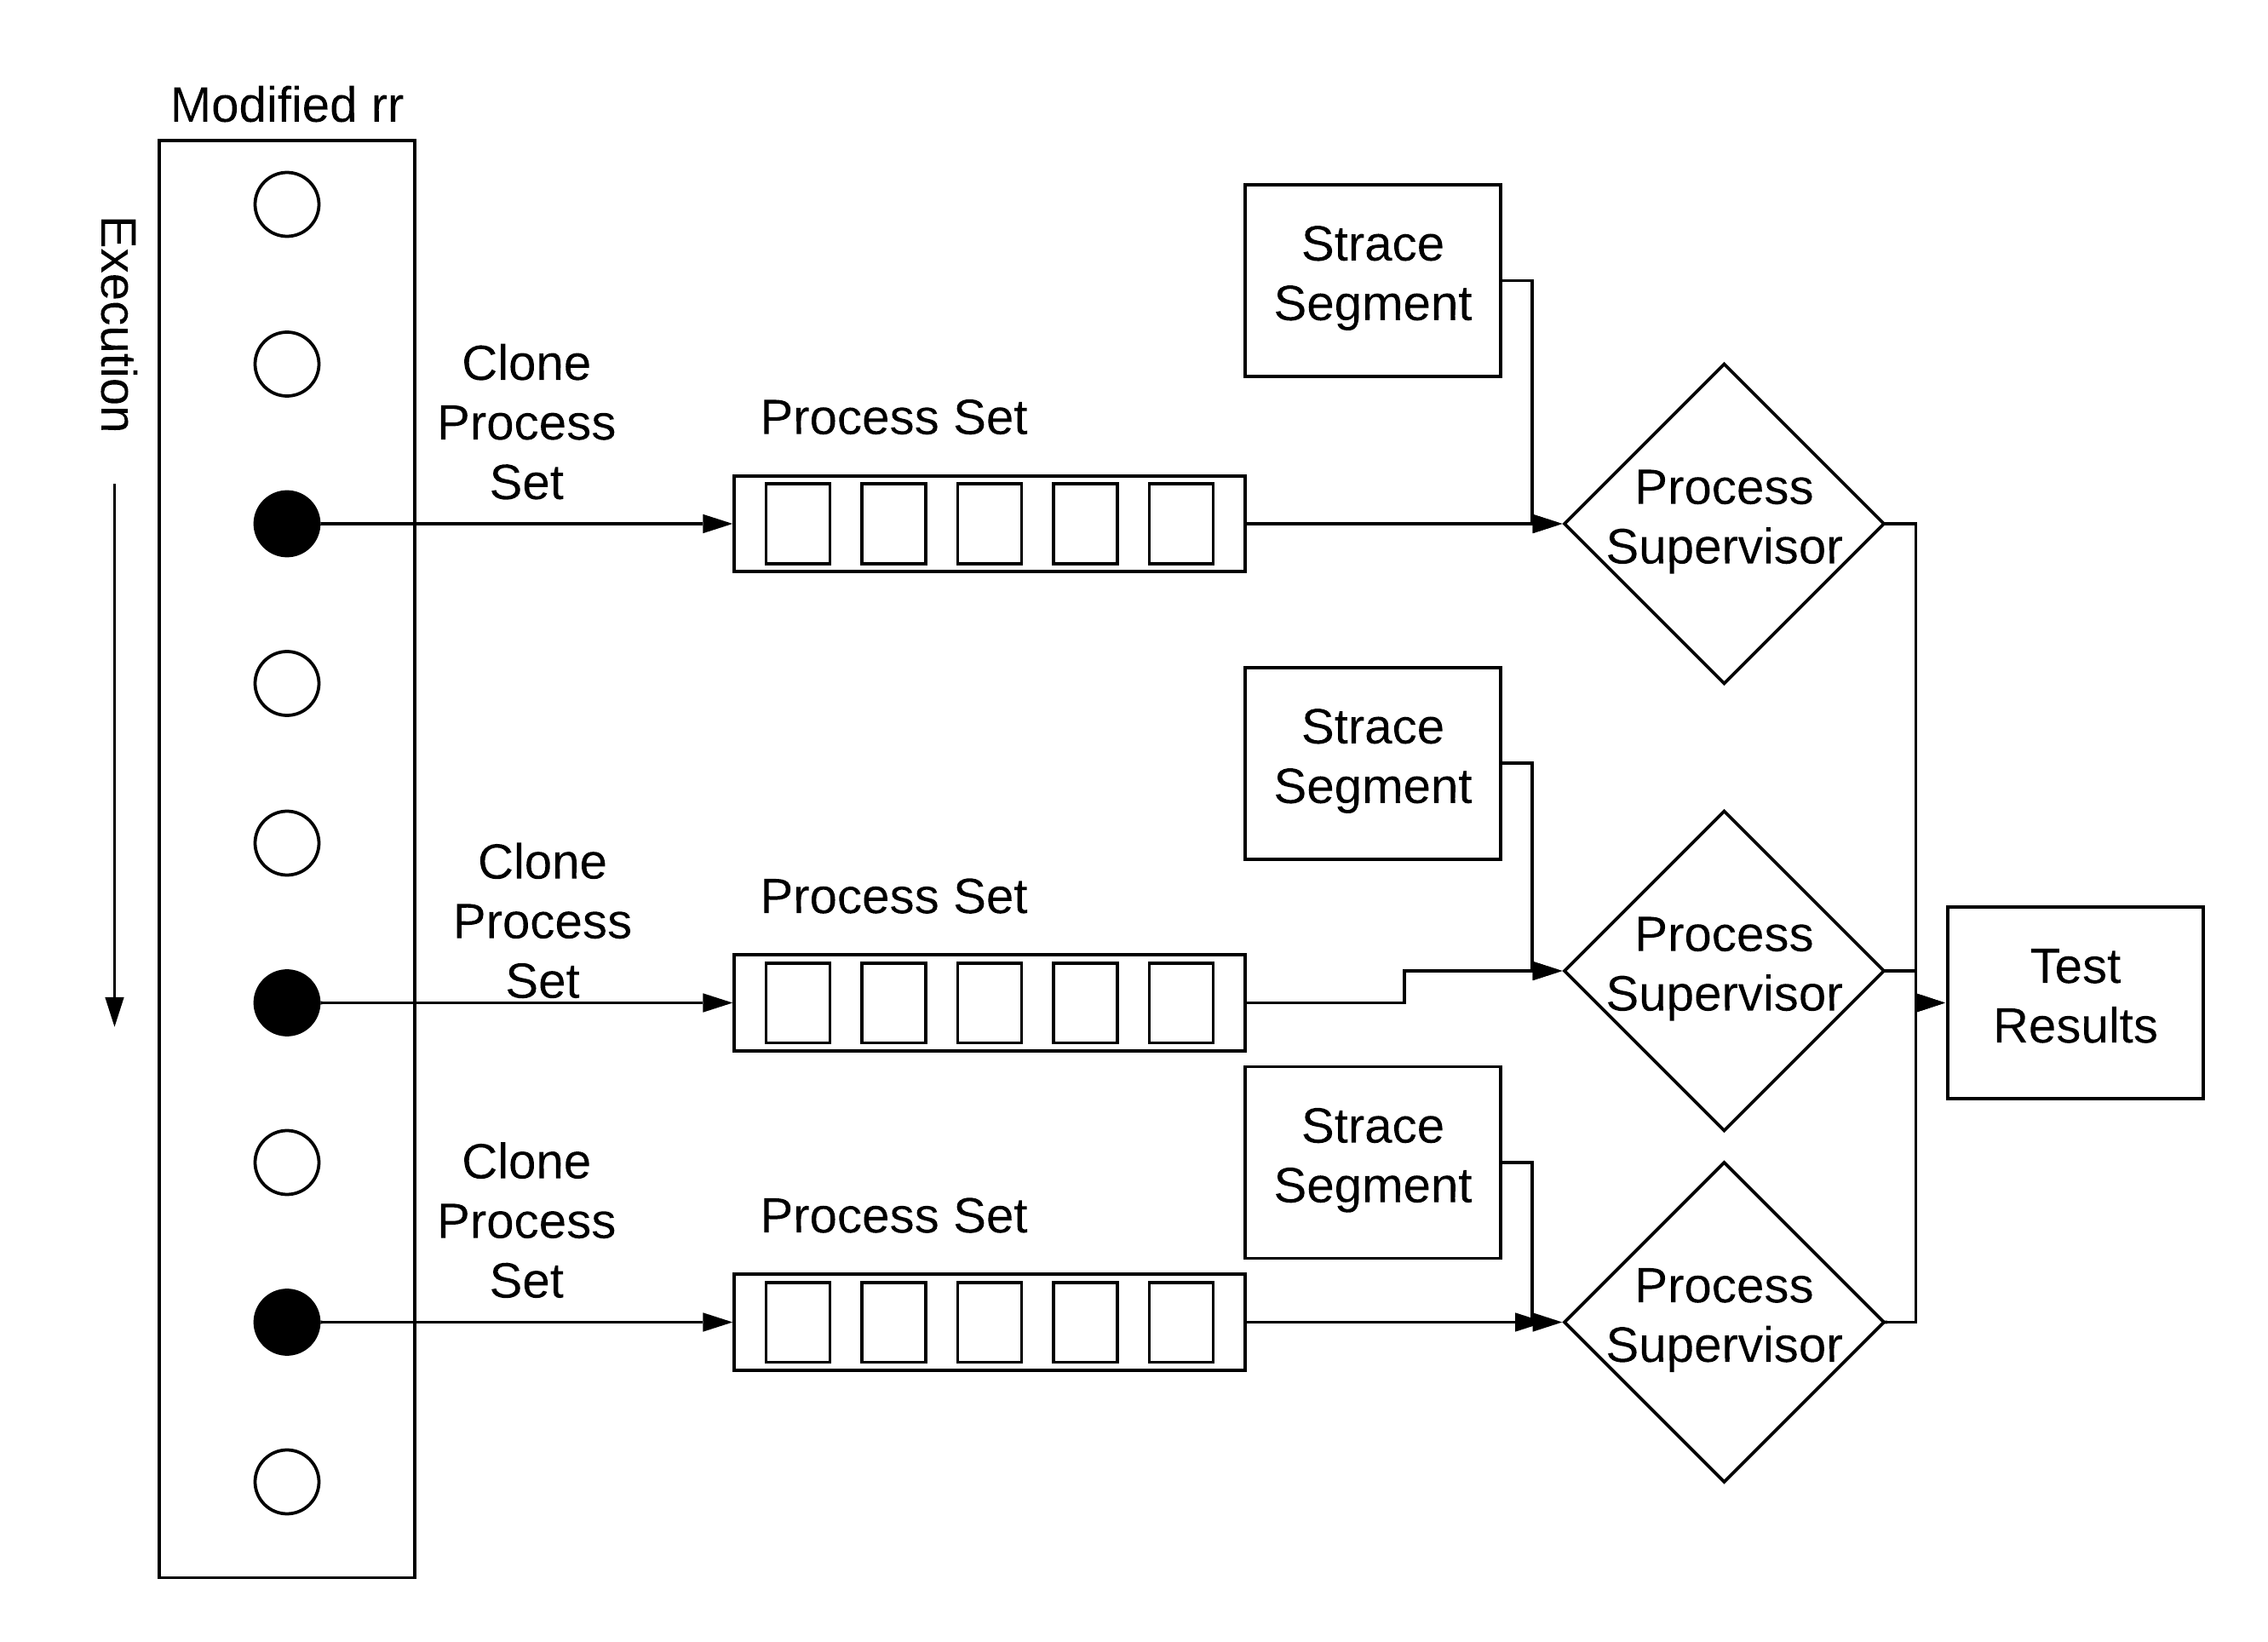
\includegraphics[width = 0.9\textwidth]{images/architecture}
  \end{figure}
\end{frame}


\begin{frame}{Architecture Discussion}
  \begin{figure}
    \centering
    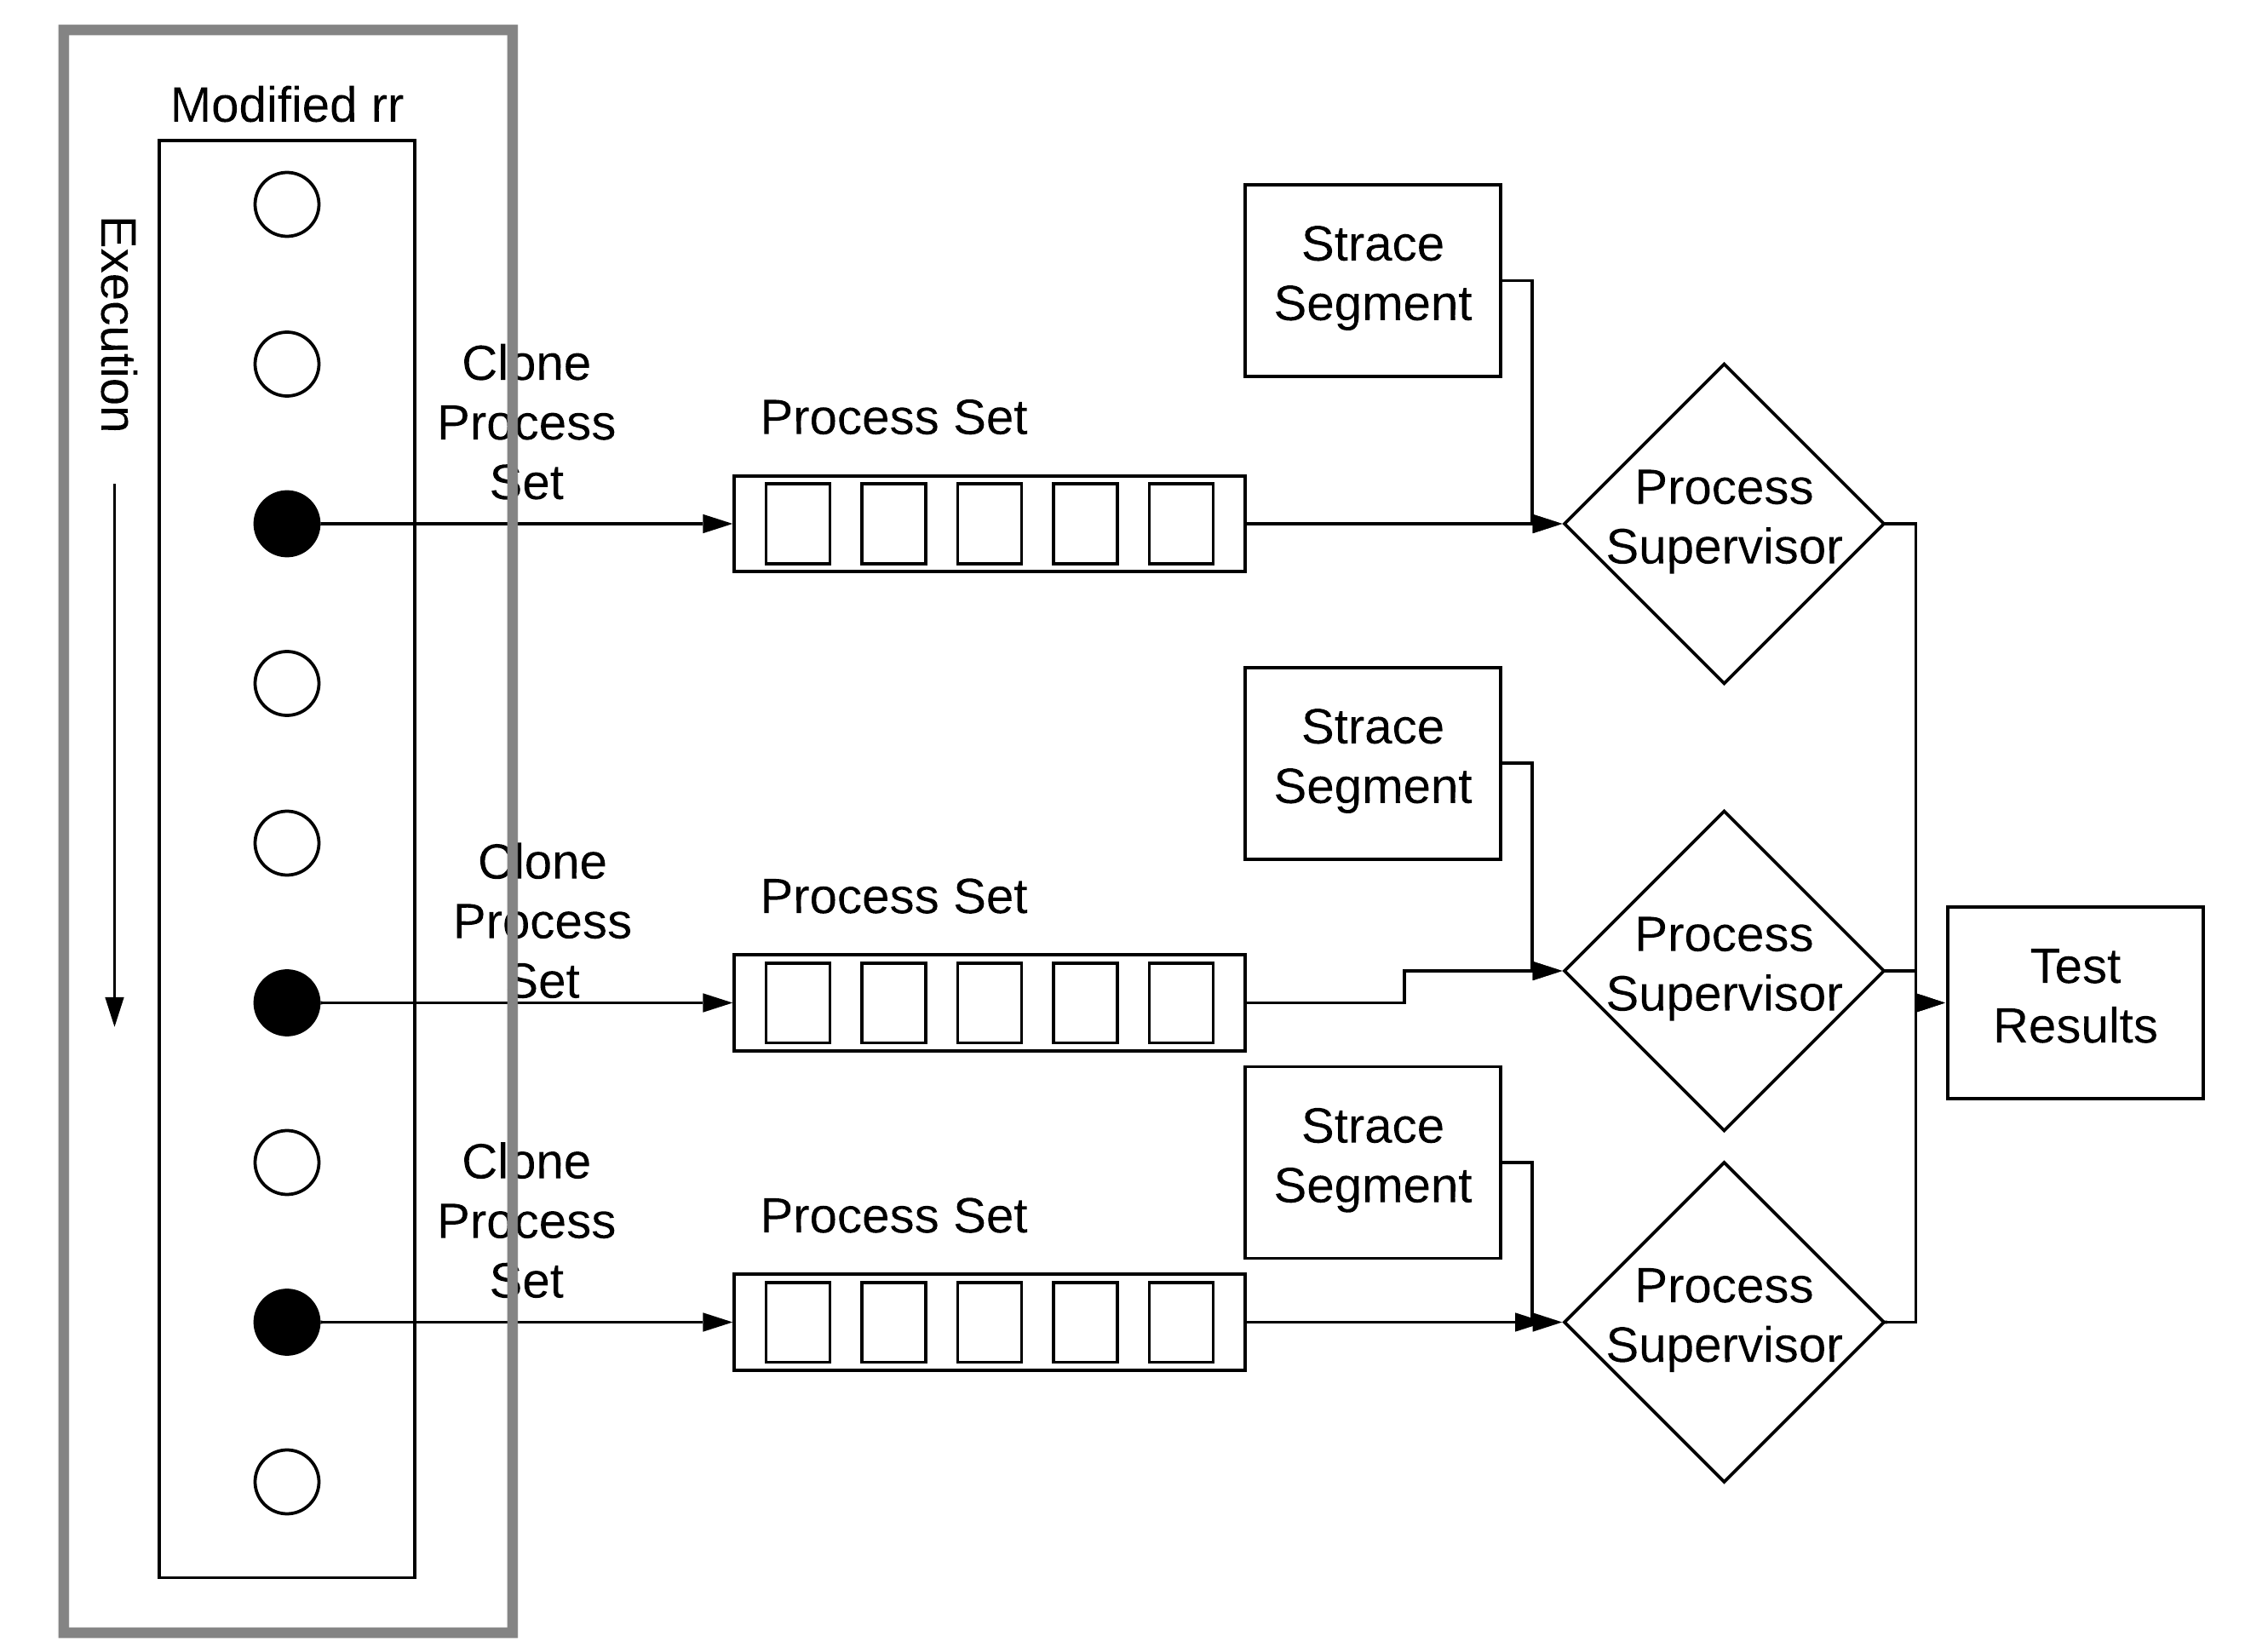
\includegraphics[width = 0.7\textwidth]{images/architecture_replay}
  \end{figure}
  \begin{itemize}
    \item{rr replays application under test until simulation opportunity
      arises}
  \end{itemize}
\end{frame}


\begin{frame}{Architecture Discussion}
  \begin{figure}
    \centering
    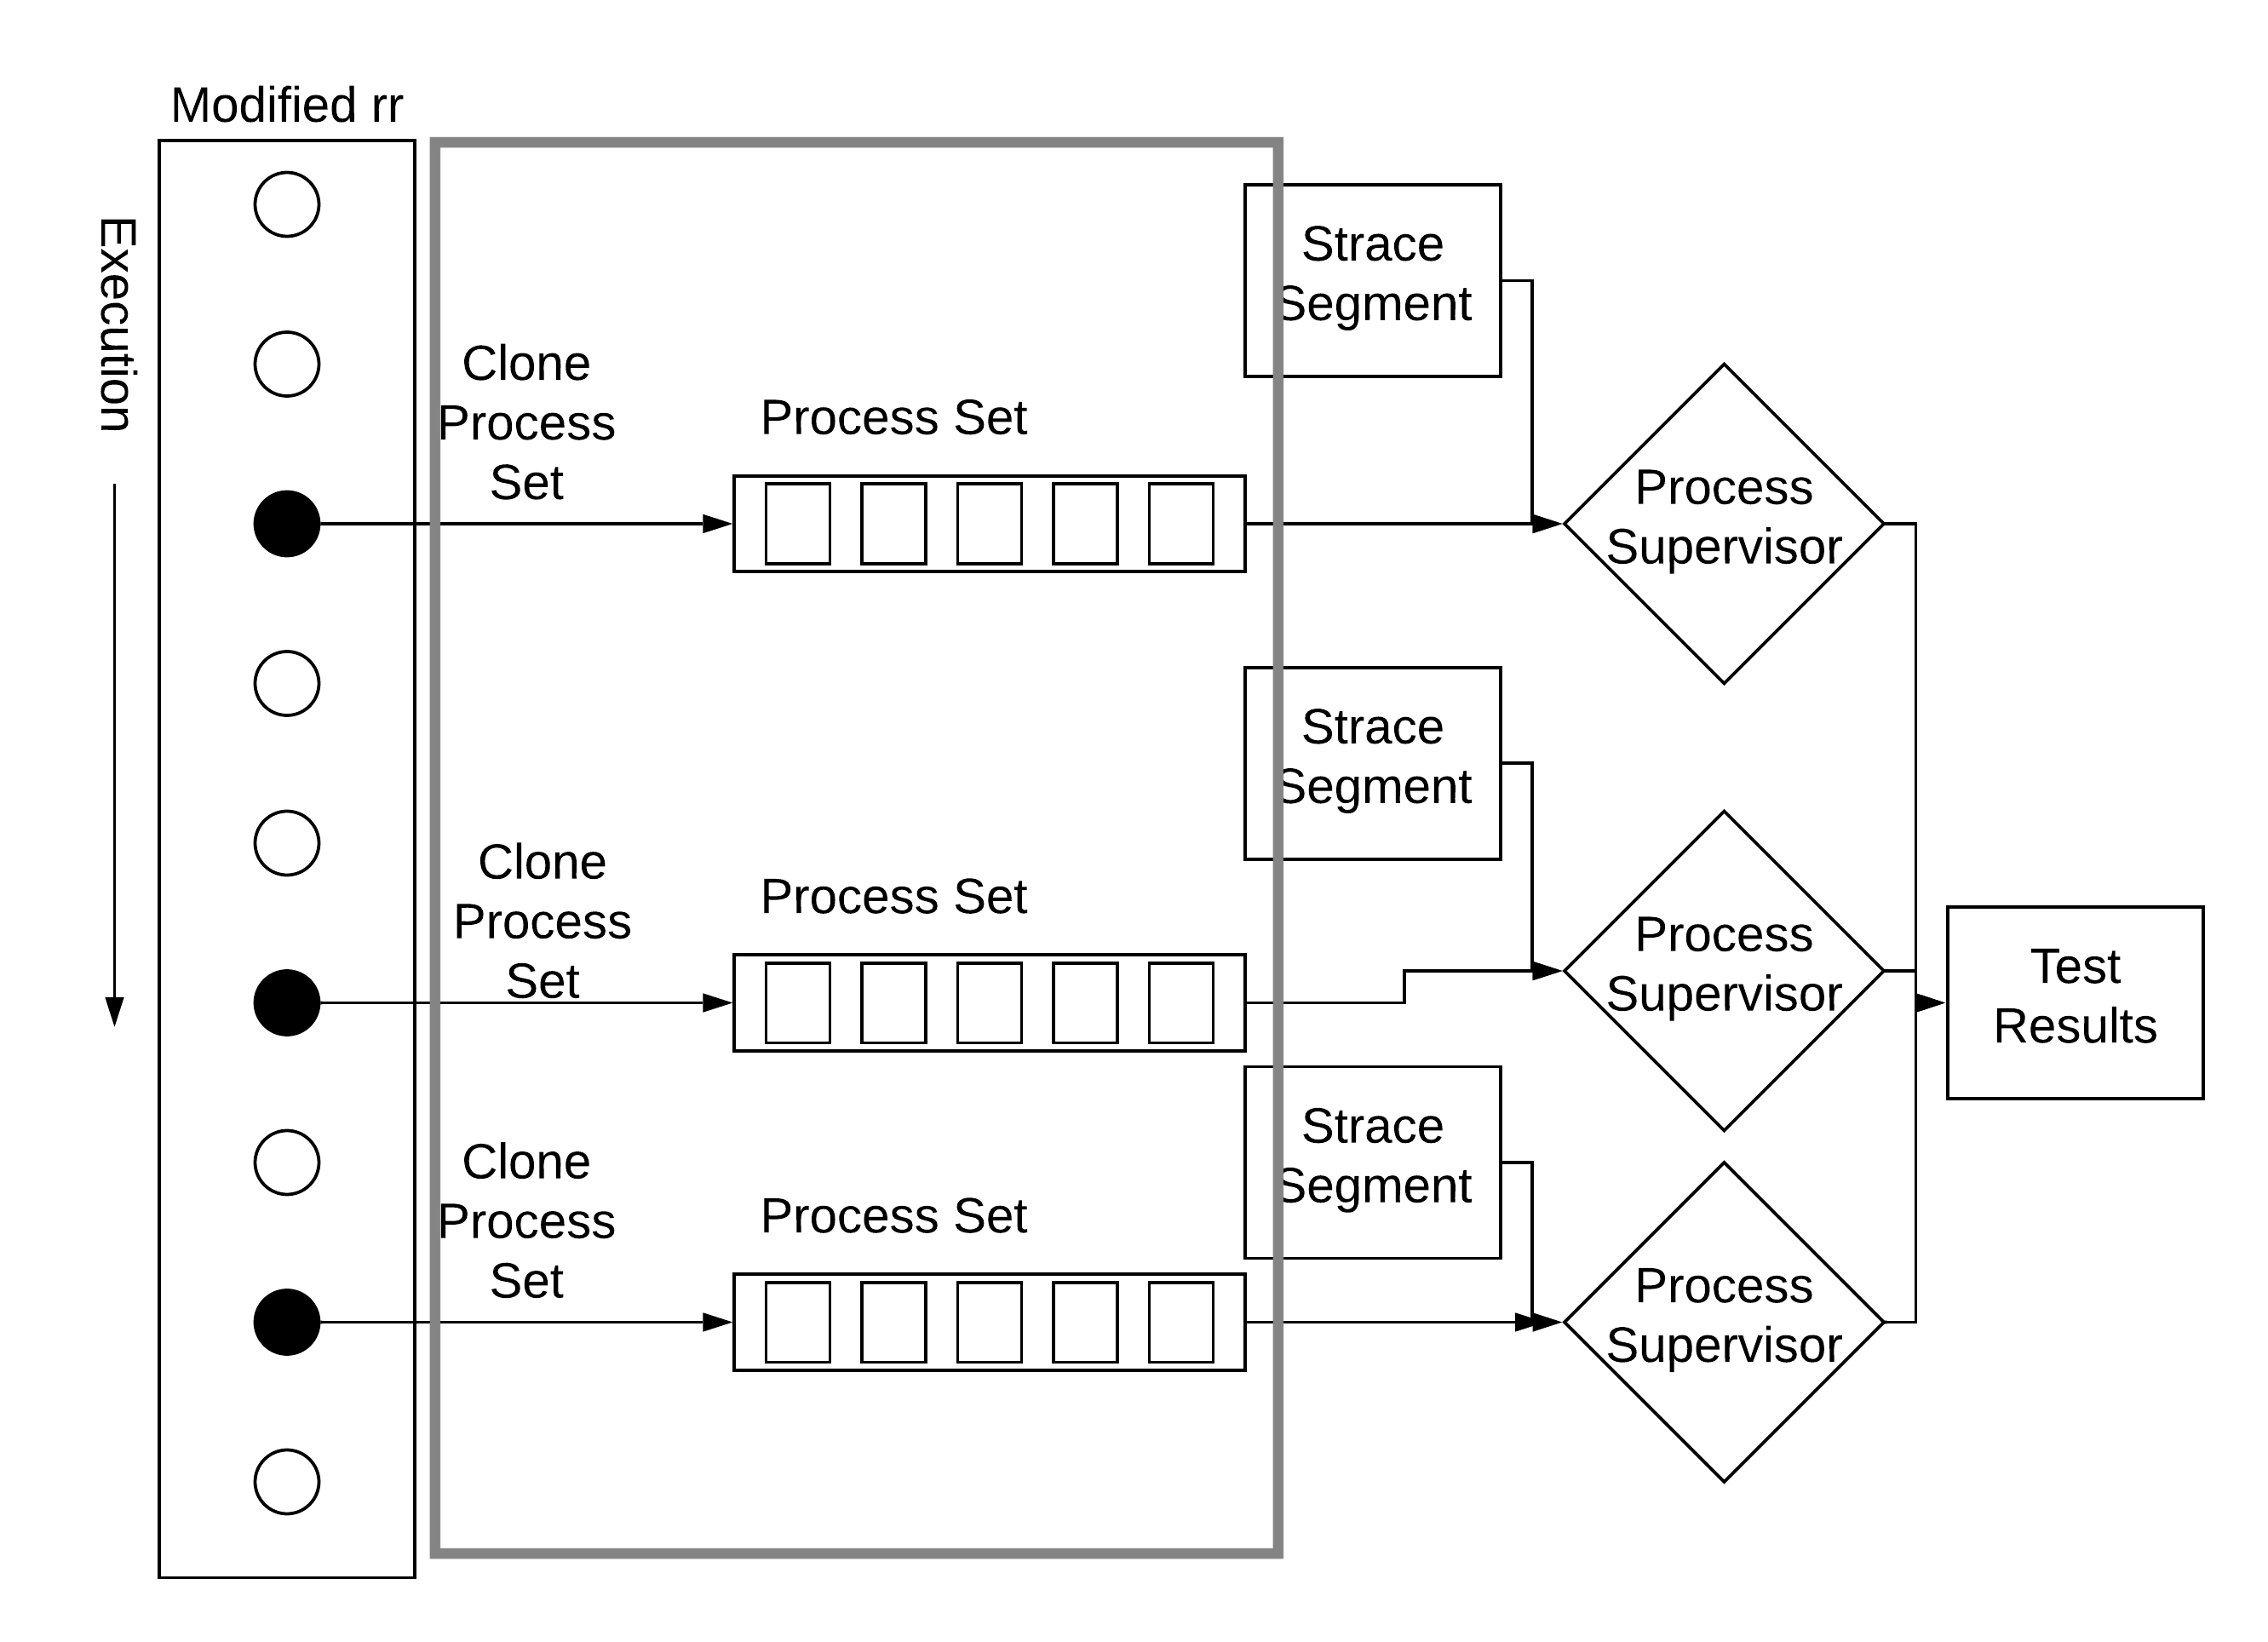
\includegraphics[width = 0.7\textwidth]{images/architecture_process_sets}
  \end{figure}
  \begin{itemize}
    \item{Modifications to rr allow complete process set of application to
      be cloned at this point}
  \end{itemize}
\end{frame}


\begin{frame}{Architecture Discussion}
  \begin{figure}
    \centering
    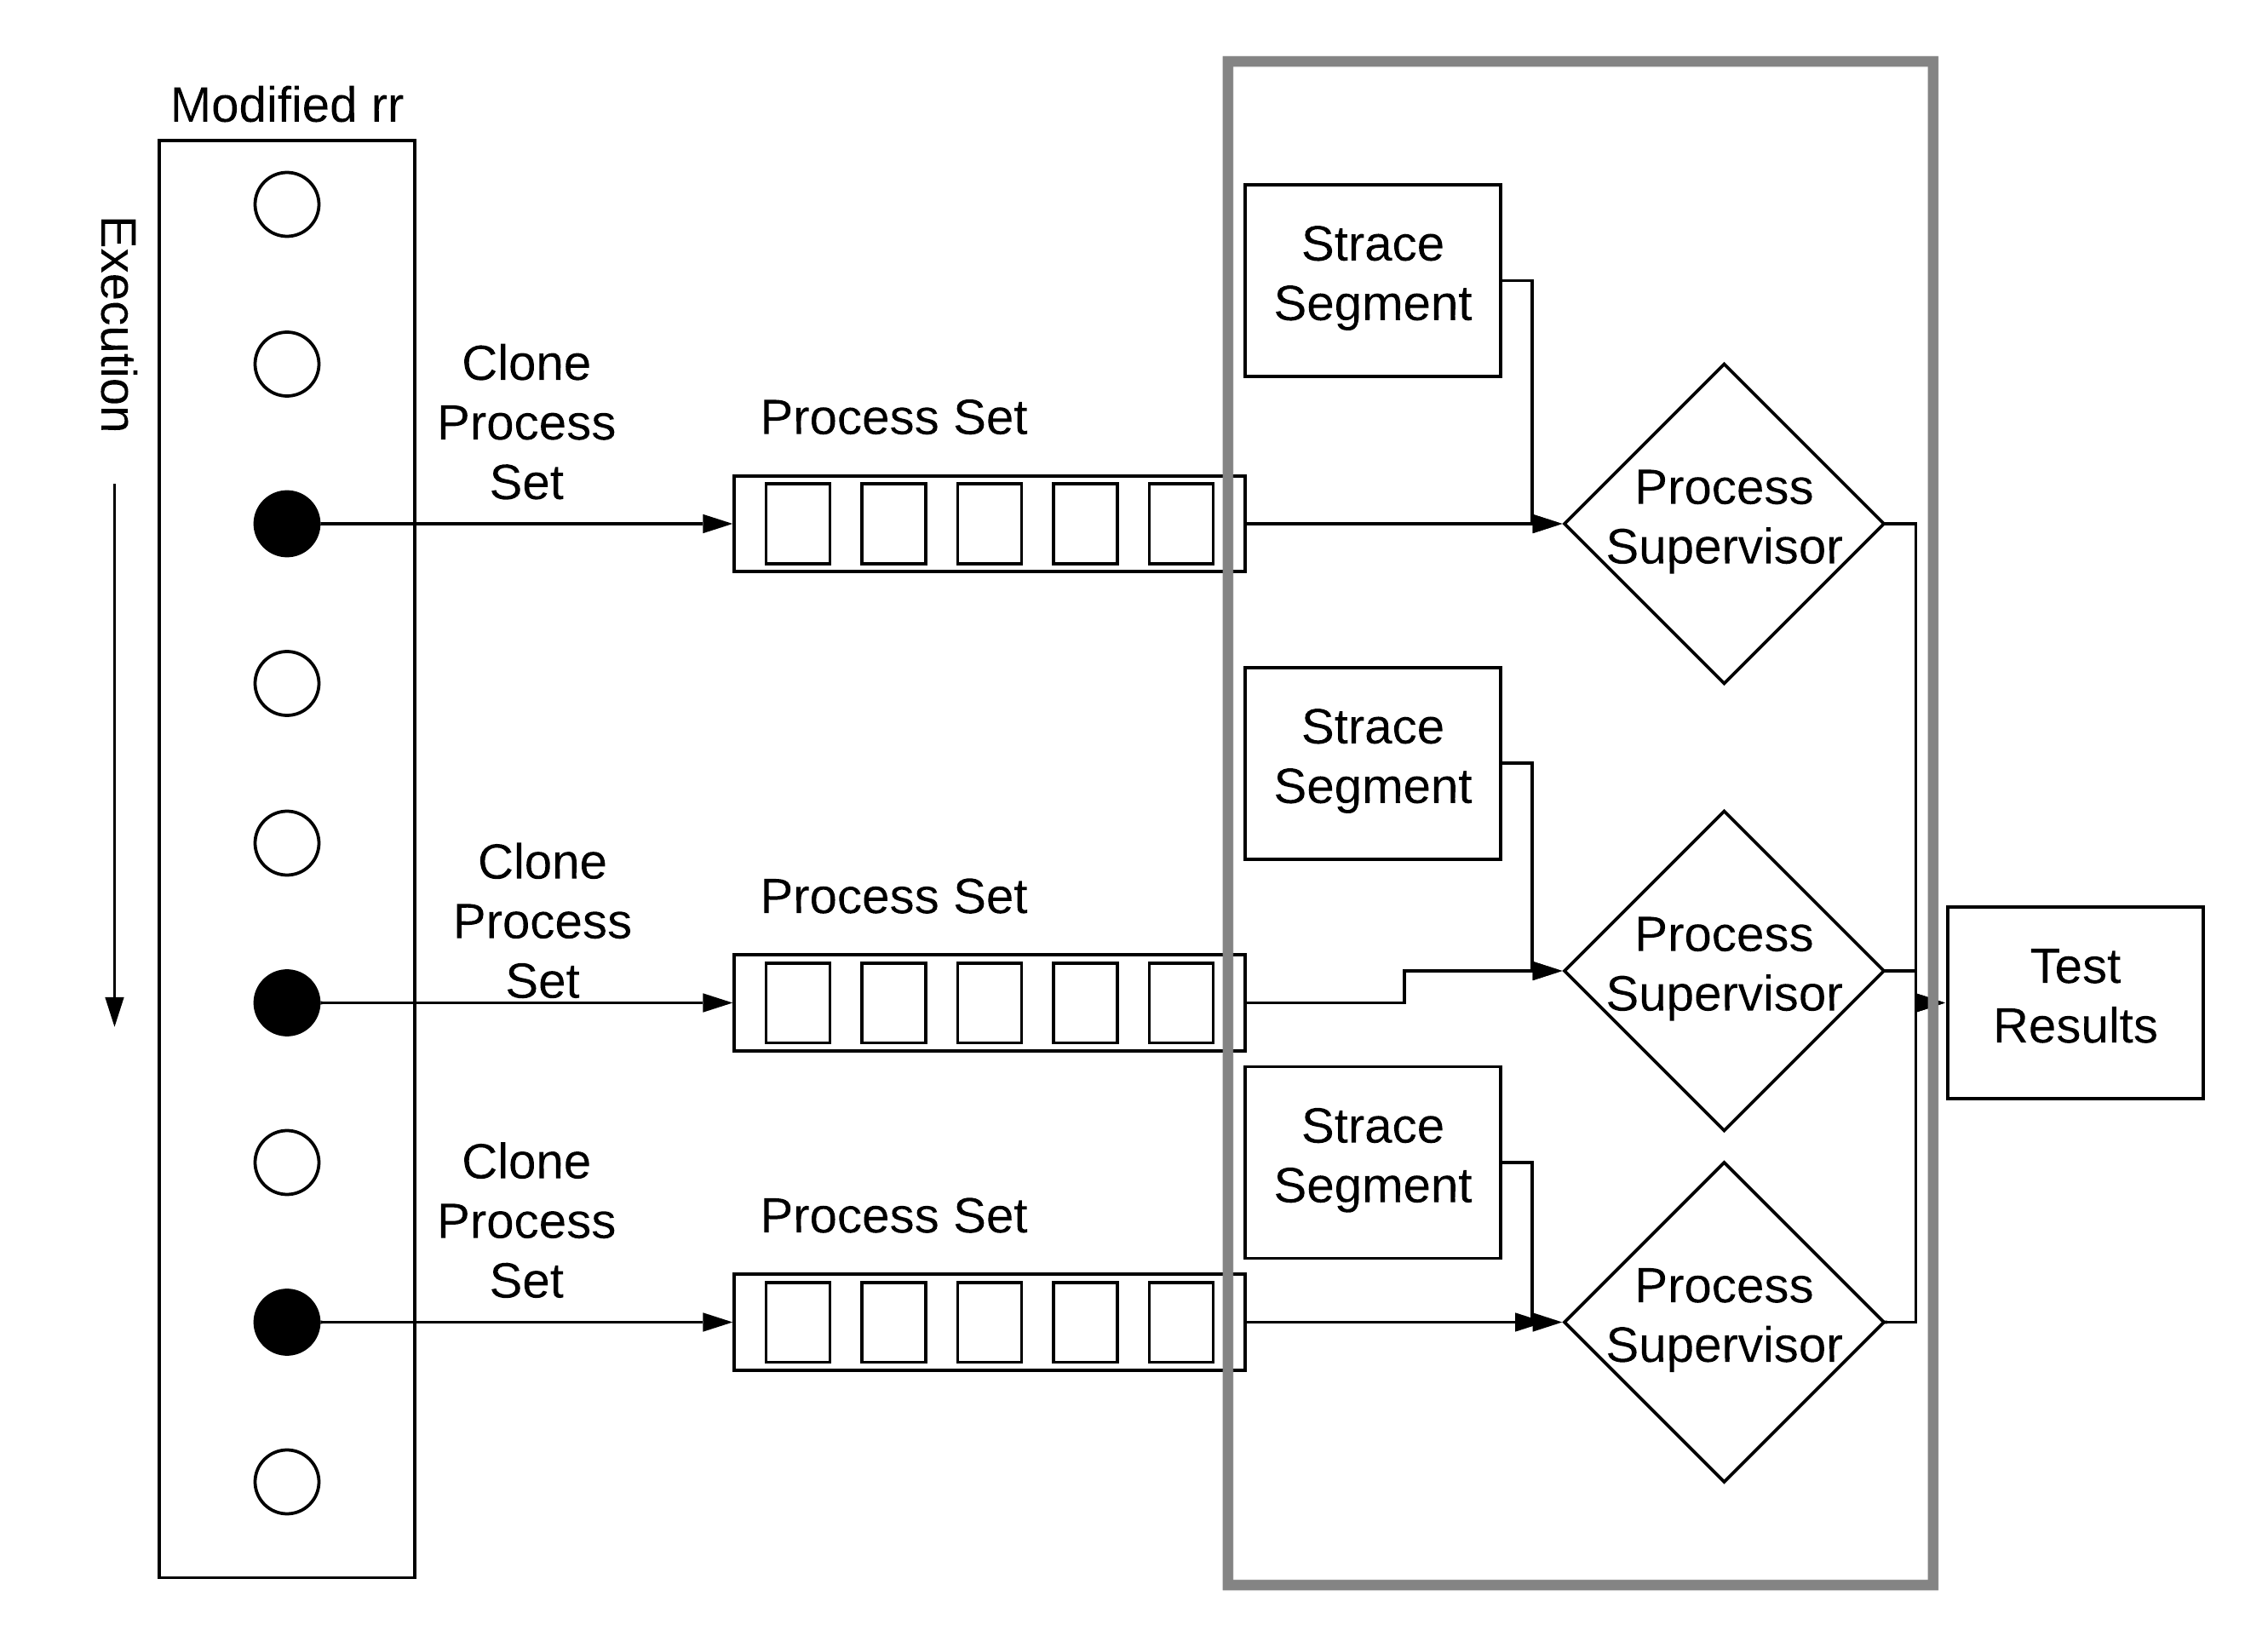
\includegraphics[width = 0.7\textwidth]{images/architecture_mutator_supervisor}
  \end{figure}
  \begin{itemize}
    \item{CrashSimulator process supervisor attaches to cloned process set
      and modifies system call results to simulate an anomaly}
  \end{itemize}
\end{frame}


\begin{frame}{Architecture Discussion}
  \begin{figure}
    \centering
    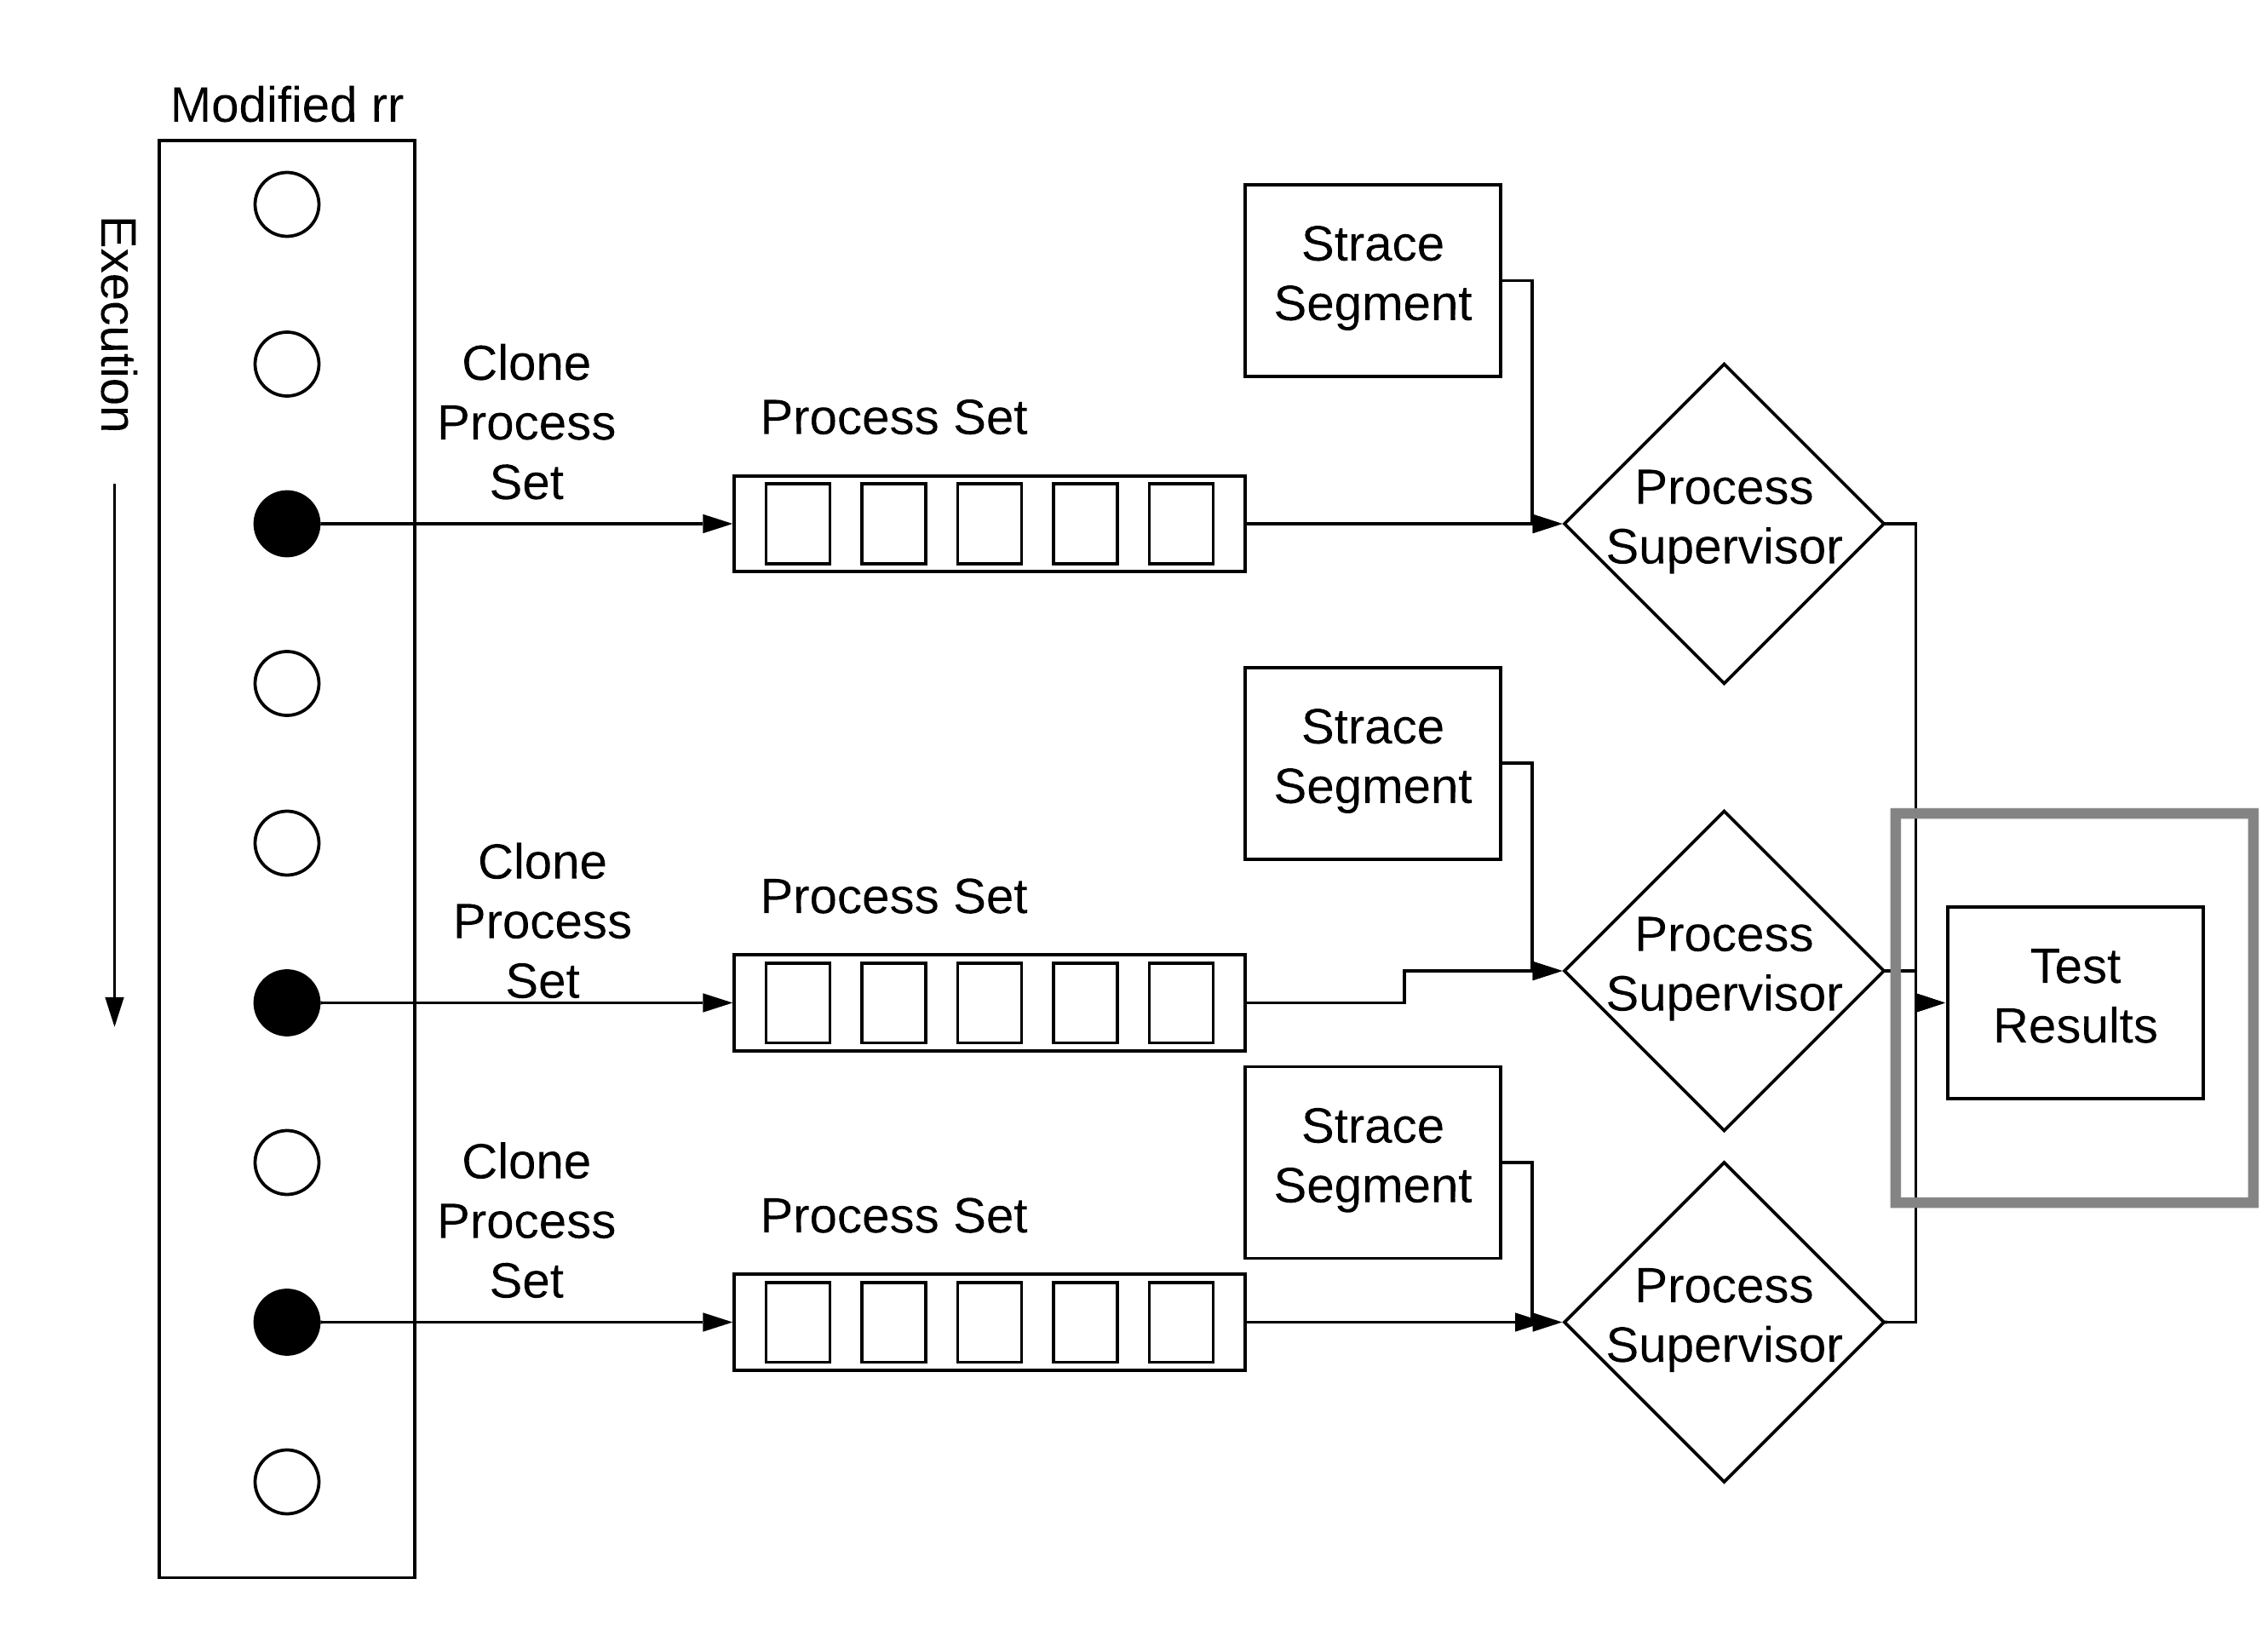
\includegraphics[width = 0.7\textwidth]{images/architecture_checker_results}
  \end{figure}
  \begin{itemize}
    \item{Checker analyzes application behavior post-simulation and reports
      results}
  \end{itemize}
\end{frame}


\begin{frame}{Evaluation Overview}
  \begin{itemize}
    \item{Unexpected Linux File Types}
    \item{Cross-disk File Movement}
    \item{Extremely Long Network Timeouts}
  \end{itemize}
\end{frame}


\begin{frame}{Eval Part 1: Unexpected Linux File Types}
  \begin{itemize}
    \item{Linux provides different types of files with different capabilities}
    \item{Application should confirm file type before processing a file}
    \item{Otherwise, problems:}
      \begin{itemize}
        \item{Applications hang on FIFOs files}
        \item{Applications consume disk space/memory/etc. processing ``infinitely
          large'' files}
      \end{itemize}
    \item{Found bugs in coreutils utilities, gnupg, and other common
        applications}
  \end{itemize}
\end{frame}


\begin{frame}{Unusual File Type Bugs}
  % Unifying subhead that shows we are working through anomalies
%\begin{table}[t]
%    \scriptsize{}
%    \begin{tabular}{l  l  |  l  l  l  l  l  l  l}
%    \toprule{}
%        Application       & Condition Tested           & Regular File           & Directory               & Character Device        & Block Device           & Named Pipe                 & Symbolic Link             & Socket File \\
%                          &                            &  (IFREG)               & (IFDIR)                 & (IFCHR)                 & (IFBLK)                & (IFIFO)                    & (IFLNK)                   & (IFSOCK)\\
%\hline
%        {\tt Aspell}      & Dictionary File            & --                     & X: \textit{FP}          & \tickmark: \textit{FN}  & X                      & X                          & X                         & X          \\
%        {\tt Aspell}      & File being checked         & --                     & X: \textit{FP}          & \tickmark               & X                      & X                          & X                         & X          \\
%        {\tt gnu-gpg}     & secring.gpg                & --                     & X                       & X                       & X                      & X                          & X                         & X          \\
%        {\tt vim}         & File being opened          & --                     & \tickmark: \textit{FN}  & \tickmark: \textit{FN}  & \tickmark: \textit{FN} & \tickmark: \textit{FN}     & \tickmark: \textit{FN}    & X          \\
%        {\tt nano}        & File being opened          & --                     & \tickmark               & \tickmark               & \tickmark              & X: \textit{FP}             & X: \textit{FP}            & X: \textit{FP} \\
%        {\tt sed}         & File being edited          & --                     & \tickmark               & X: \textit{FP}          & X                      & X                          & X                         & X          \\
%        {\tt wc}          & File being checked         & --                     & \tickmark               & X                       & X                      & X                          & X                         & X          \\
%        {\tt du}          & Directory being checked    & \tickmark              & --                      & \tickmark               & \tickmark              & \tickmark                  & \tickmark                 & \tickmark  \\
%        {\tt install}     & File being installed       & --                     & \tickmark               & X                       & X                      & X                          & \tickmark                 & X          \\
%        {\tt fmt}         & File being formatted       & --                     & X                       & \tickmark               & X                      & X                          & X                         & X          \\
%        {\tt od}          & File being dumped          & --                     & \tickmark               & \tickmark               & X                      & X                          & X                         & X          \\
%        {\tt ptx}         & File being read            & --                     & \tickmark               & \tickmark               & \tickmark              & \tickmark                  & \tickmark                 & \tickmark: \textit{FN} \\
%        {\tt comm}        & Second file being compared & --                     & \tickmark               & \tickmark               & X                      & X                          & X                         & X          \\
%        {\tt pr}          & File being read            & --                     & \tickmark               & X                       & X                      & X                          & X                         & X          \\
%\hline
%        \multicolumn{9}{l}{\scriptsize{\tickmark  $=$ CrashSimulator
%        predicts application will recognize anomaly}}\\
%        \multicolumn{9}{l}{\scriptsize{X $=$ CrashSimulator predicts
%        application will fail to recognize anomaly}}\\
%        \multicolumn{9}{l}{\scriptsize{-- $=$ File type expected by the
%        application}}\\
%    \bottomrule{}
%    \end{tabular}
%    \setlength{\belowcaptionskip}{-13pt}
%\end{table}
  This table is much to wide to fit onto a slide.  Not sure how best to
  include this data...
\end{frame}


\begin{frame}{Unusual File Types Case Study: Aspell Bug}
  \begin{itemize}
    \item{Aspell did not resolve destination of symlinks before operating
      on them.}
    \item{Passing a symlink to /dev/urandom crashed application and filled
      disk with garbage}
    \item{Discovered by simulating presence of symlink rather than regular
      file}
    \item{Patch submitted and accepted}
  \end{itemize}
\end{frame}


\begin{frame}{Unusual Filetypes - The Takeaway}
  % Unifying subhead that shows we are working through anomalies

  \begin{itemize}
    \item{We learned that applications fail to diligently check file types
        before operating on files}
    \item{Developers should perform these checks or rely on libraries that
        make these checks for them}
  \end{itemize}
\end{frame}


\begin{frame}{Eval Part 2: Extremely Long Network Timeouts Discussion}
  % Move network timeout bugs to be the middle item of discussion because
  % we don't have a real example to talk about making it weaker from a
  % presentation perspective

  % Unifying subhead that shows we are working through anomalies

  % Shorten the sentences while keeping the points to make this slide
  % shorter

  % Break this up into smaller slides
  \begin{itemize}
    \item{Applications that do not configure reasonable timeouts are vulnerable
      to a malicious communication participant dragging communication out over a
      long period of time}
    \item{This process ties up resources and makes DoS easier}
    \item{``Slowloris'' Denial of Service attack against http servers}
      \begin{itemize}
        \item{involves keeping a connection open to a vulnerable server by
          introducing just-below-the-timeout delays between sending HTTP headers}
      \end{itemize}
   % \item{MANY Python HTTP/HTTPS/web modules vulnerable}
  \end{itemize}
\end{frame}


\begin{frame}{Extremely Long Network Timeouts Results}
  % Unifying subhead that shows we are working through anomalies
\begin{table}[t]
  \scriptsize{}
  \begin{tabular}{l | l}
    \toprule{}
    {\bf Application}              & {\bf Analysis Result}\\
    {\tt wget}                     & Overly long timeout supplied to {\tt select()} \\
    {\tt ftp}                      & No {\tt poll()} or {\tt select()}, no timeout set \\
    {\tt telnet}                   & {\tt select()} specifies no timeout \\
    {\tt urllib http}              & No {\tt poll()} or {\tt select()}, no timeout set \\
    {\tt urllib ftp}               & No {\tt poll()} or {\tt select()}, no timeout set \\
    {\tt ftplib}                   & No {\tt poll()} or {\tt select()}, no timeout set \\
    {\tt httplib}                  & No {\tt poll()} or {\tt select()}, no timeout set \\
    {\tt requests}                 & No {\tt poll()} or {\tt select()}, no timeout set \\
    {\tt urllib3}                  & No {\tt poll()} or {\tt select()}, no timeout set \\
    {\tt python-websocket-client}  & No {\tt poll()} or {\tt select()}, no timeout set \\
    \bottomrule{}
  \end{tabular}
\end{table}
\end{frame}


\begin{frame}{Extremely Long Network Timeouts - The Takeaway}
  \begin{itemize}
    \item{Major applications and libraries are vulnerable to maliciously
      timed communications}
    \item{Assumption that ``users will do it'' falls flat}
    \item{Users should configure libraries with reasonable timeouts}
    \item{Libraries should consider shorter defaults}
  \end{itemize}
\end{frame}


\begin{frame}{Eval Part 3: Cross-Disk File Movement Discussion}
  % Unifying subhead that shows we are working through anomalies

  % Maybe split this content out over two slides
  \begin{itemize}
    \item{Moving a file around on the same disk is trivial: rename() system
      call}
    \item{This system call does not support moving a file from one disk to
      another}
    \item{An application must detect this situation and either fail
      gracefully or perform the file move ``manually''}
  \end{itemize}
\end{frame}


\begin{frame}{Eval Part 3: Cross-Disk File Movement Discussion}
    % Cross-filesystem rather than cross disk?
    \begin{itemize}
    \item{Otherwise, problems:}
      \begin{itemize}
        \item{Loss of file contents}
        \item{Loss of file metadata}
        \item{Race conditions}
        \item{Filling of disk space}
      \end{itemize}
    \item{Race condition in Python's shutil}
    \item{Loss of extended file attributes in Rust's std::fs}
    \item{Fill disk space bug in C++'s Boost::filesystem}
  \end{itemize}
\end{frame}


\begin{frame}{Cross-Disk File Movement Results}
  % Unifying subhead that shows we are working through anomalies
 \begin{table}[t]
    \scriptsize{}
    \begin{tabular}{l p{1cm} p{1cm} p{1.2cm} p{1cm}}
    \toprule{}
        Application     & Source Replaced & Preserve Xattrs & Preserve Timestamps & Copying Devices\\
\hline
        {\tt mv}              & Correct             & Correct         & Correct             & Correct\\
        {\tt mmv}             & Correct             & {\bf Sec. Flaw} & {\bf Time Loss} & Correct\\
        {\tt install}         & Correct             & {\bf Sec. Flaw} & {\bf Time Loss} & {\bf Fill Disk} \\
        {\tt perl File::Copy} & Correct             & {\bf Sec. Flaw} & {\bf Time Loss} & {\bf Fill Disk} \\
        {\tt shutils}         & {\bf Corrupt}	& {\bf Sec. Flaw} 	& Correct             & Correct\\
        {\tt rust}             & Correct             & {\bf Sec. Flaw} & {\bf Time Loss} & {\bf Fill Disk} \\
        {\tt boost::copyfile} & {\bf Corrupt}	      & {\bf Sec. Flaw} & {\bf Time Loss} & {\bf Fill Disk} \\
    \bottomrule{}
    \end{tabular}
\end{table}
\end{frame}


\begin{frame}{Cross-Disk File Movement Case Study: shutil race condition}
  \begin{itemize}
    \item{shutil.copyfile() fails to save and check file inode before
      copying it}
    \item{File can be replaced during move: security issue}
    \item{Detected with Cross-Disk move checkers and Null Mutator}
    \item{Patch submitted, fix in progress}
  \end{itemize}
\end{frame}


\begin{frame}{Cross-Disk File Movement - The Takeaway}
  \begin{itemize}
    \item{Well known, popular applications are not moving files correctly}
    \item{Developers should use libraries that handle these cases
        correctly}
  \end{itemize}
\end{frame}



% Maybe a future work slide here

\begin{frame}{In Conclusion}
  \begin{itemize}
    \item{An application's environment is an often-neglected cause of bugs}
    \item{These bugs are difficult to find pre-deployment because replicating
      unusual environments is expensive}
    % Hard to find because there are too many environment combinations to
    % to test against
    \item{SEA helps find these bugs by simulating problematic environmental
        features in order to identify bugs before deployment}
    \item{Our implementation of SEA, CrashSimulator, has found these types
      of environmental bugs in both popular applications and libraries}
  \end{itemize}
\end{frame}

% Future work slide

\end{document}
